\section{Phases of Venus}


One of the most important things Galileo observed with his telescope is that
Venus has phases like the Moon.   This was the ``smoking gun'' that showed
that the earth-centered (pre-Copernicus) system couldn't possibly be right,
so it went a long way toward convincing people that the Earth really did
go around the Sun.  We're going to examine the phases of Venus to see what
Galileo saw and why it mattered. You can do this lab using either
\textit{Stellarium} or \textit{Sky Safari}.

Start up your program of choice.
Turn off 
the effects of Earth's atmosphere (daylight) and 
make the ground transparent,
so that it's possible to see the stars and planets all the time.
Use the equatorial (stationary-sky) point of view.
Set the view to be centered on the Sun.

Keep the view centered on the Sun, and let time run forwards and backwards 
at high speed for a year or two.
Observe
motion of Venus.  Note that it swings back and forth past the Sun,
never getting more than a certain angular separation from the Sun in the sky.

Here's one preliminary question before we look at the phases of Venus.  If
you wanted to observe Venus today, at what time of night should you observe?
Specifically, find a rough time when Venus is above the horizon but the Sun
is below the horizon.  

Best time to observe Venus these days:

\answerspace{0.7in}

What if you wanted to observe Venus on August 20? When would be the
best time to see it?

\answerspace{0.7in}

What about on September 20?

\answerspace{0.7in}


If you had to choose one of those three dates on which to observe
Venus, which one would be best? Which would be worst?

\answerspace{0.7in}

Venus spends quite a bit of its time vey near the Sun in the sky,
at which times it's hard to observe.
The easiest time to observe Venus is when its as far away from
the Sun in the sky as possible.  This is called the time of ``maximum
elongation.''  Set the time back to today, 
and run time forwards until you find the next time of maximum
elongation.  (Don't worry about being incredibly precise; if you're
within about a week or so of the correct date, that's fine.)
Find the angular
separation between
Venus and the Sun at that time. 

Maximum angular separation between Sun and Venus:

\answerspace{0.7in}

\pagebreak[3]

Here's a diagram showing the Earth's and Venus's orbits around the
Sun.  Suppose that the Earth is at the uppermost point in its orbit as
shown, and suppose that Venus is at maximum elongation from the Sun
(so that it appears as far from the Sun as possible in the sky).  Draw
a circle to mark the position of Venus in its orbit.  (There are
actually two possibilities.  One corresponds to the case where Venus
is to the East of the Sun and one to the case where it's to the West.
If you assume everything orbits
counterclockwise, you can figure out which which, although
it's a bit tricky.  For the moment, it doesn't matter which one you choose.)

\begin{figure}[h]
%\centerline{\epsfxsize 3in\epsfbox{figs/venus1.eps}}
\centerline{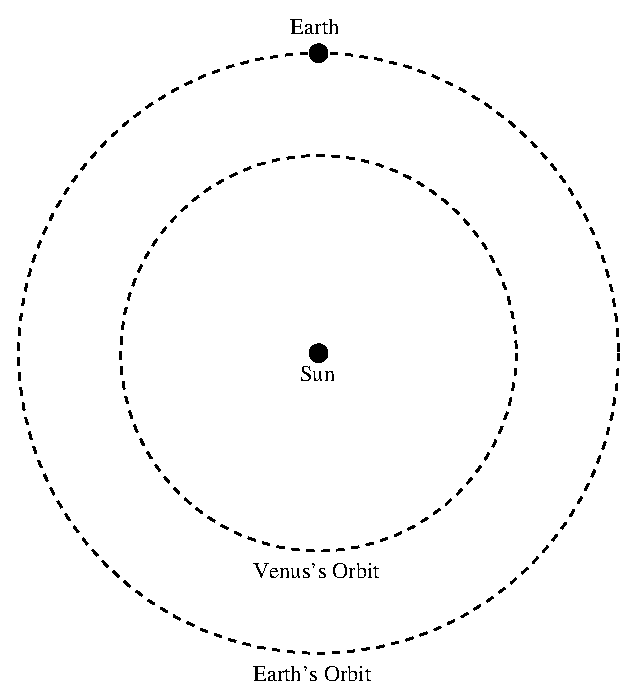
\includegraphics[width=3in]{phasesofvenus/venus1.eps}}
\end{figure}


Venus, like the Moon, shines by reflected sunlight.  That means that
the only part of Venus we'll see is the part that's illuminated by the 
Sun.  In the diagram above, shade in the half of Venus that's lit up by
the Sun, and then use the diagram to predict the phase of Venus
at this time.  (That is, will Venus appear like a crescent, like
a ``full'' Venus, or what?)

\answerspace{0.6in}

After you've made your prediction, use \textit{Stellarium}
or \textit{Sky Safari}  to test it.
Center the view on Venus and zoom in to enlarge the image of Venus.
Does it have the phase you predicted?

\answerspace{0.6in}

Now set the date to July 20, and 
zoom in on Venus to observe its phase.  What is the phase of Venus on that date?

\answerspace{0.6in}

\pagebreak[2]

Based on your observation, is Venus in front of the Sun or behind the Sun
on that date?

\answerspace{0.7in}

Zoom back out again, and center the field of view on the Sun.  Let time
run forward until Venus has gone through about half of one orbit.  You
should see it pass by the Sun, go out to maximum elongation, and then come
back until it approaches near the Sun again.  At this point, when
Venus's path is about to cross past the Sun again, is Venus in front
of the Sun or behind the Sun?  (Don't use the program to answer this; 
use what you know about the orbits.)

\answerspace{0.7in}

Based on your answer to the previous question, what do you expect the 
phase of Venus to be?

\answerspace{0.7in}

What do you expect about the angular size of Venus: should it be bigger
or smaller than the last time you looked at it?

\answerspace{0.7in}

Now use \textit{Stellarium} or \textit{Sky Safari} to
test these predictions.
Center the view on Venus and zoom in.
Were your predictions right?

\answerspace{0.7in}

Keep the field of view centerd on Venus and zoomed all the way in.  Let time
run forward fast for a year or two.  The main things to note are that
Venus goes through a full set of phases (from crescent to full and back),
and that its angular size changes along with its phase.

\pagebreak[3]

Earlier, I said that this observation provided strong proof that
the old Earth-centered theory was wrong.  Let's see why.  Remember that
in the old theory the Earth was at the center, the Sun went around the
Earth, and Venus moved on an epicycle between the Earth and the Sun like this:


%\centerline{\epsfxsize 3in\epsfbox{figs/venus2.eps}}
\centerline{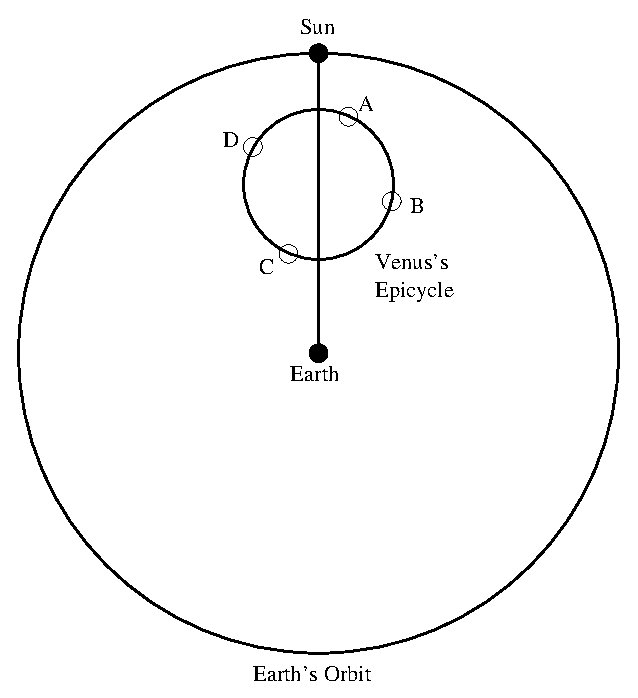
\includegraphics[width=3in]{phasesofvenus/venus2.eps}}


At each of the points A,B,C,D in the diagram, what would the phase
of Venus be, according to this model?

A:

B:

C: 

D:

What phases of Venus would {\it never} occur in the earth-centered
model?

\answerspace{0.7in}

The fact that Venus is observed to have those phases is the ``smoking
gun'' I referred to.

One more thing.  Now that you've measured the maximum elongation of
Venus, you can use it to figure out the radius of Venus's orbit.
Sketch a picture showing Earth, Sun, and Venus at the moment of 
maximum elongation (this will look the same as the diagram on the
second page of this lab).  

\answerspace{2.0in}

\pagebreak[2]

Connect these three bodies with straight lines to form a triangle.
When Venus is at maximum elongation, this triangle will have a right
angle at Venus.  The angle at the Earth is the angular separation
between Venus and Sun (that is, the angle you determined on the second page).
Indicate both of those angles on the diagram.

We also know the length of one side of the triange: the distance from
the Earth to the Sun is 1 AU.  Mark this on your triangle as well.

Now you have a right triangle, and you know one angle (other
than the right angle) and one side.
That means you can use trigonometry to find the lengths of the
other sides.  Determine the radius of Venus's orbit trigonometrically.
(If you don't remember how to do this, ask me.)



